% For instructions,
\documentclass[reprint, amsmath, amssymb, aps]{revtex4-2}

%\usepackage[norsk]{babel}
%Uncomment this if you want to write in Norwegian

\usepackage{graphicx}% Include figure files
\usepackage{dcolumn}% Align table columns on decimal point
\usepackage{bm}% bold math
\usepackage{hyperref}% add hypertext capabilities
\usepackage{booktabs}
\usepackage{float}
\usepackage{siunitx}

\renewcommand{\vec}[1]{\mathbf{#1}} %ny definisjon av \vec så det blir bold face i stedet for vector-pil.

\newcommand{\zetaR}{\tilde{\zeta}_R}

\usepackage{nicematrix}

\begin{document}
\title{Project 4 - Flow in nanoporous media using perculation theory}
\author{Mikkel Metzsch Jensen}

\date{\today}
\maketitle
\section{Defining flow}
We can adress the flow either as an incompresible fluid flowing through the porous system or in the form om electric current. It can be shown that the physcis of these are similar and there are no need to distinguish beetween these two. This i briefly explained in the following sections

\subsection{Electrical condutivity}
We assume that a voltage $V$ is applied over across the nanoporous material, such as a bond-perculation network (almost similar to site-perculation network), and the total currrent $I$, trough the sample is measured, given the conductance $G$ of the sample as the constant proportionality:
\begin{align*}
  I = GV
\end{align*}
For an $L^d$ sample the conductance $G$ of homogeneous material with conductivity $g$ is
\begin{align}
  G = L^{d-1} \frac{g}{L} = L^{d-2}g
  \label{eq:G_electric}
\end{align}
The conductance is inversely proportional to the length of the sample in the direction of flow and proportional to the cors-sectional d-1-dimensional area. We can understand this by considering that there are $L^{d-1}$ parallel parts that conribute to the flow. In addition, each part has a length $L$, and we recall from electromagnetism that conductance decrease with length.
\subsection{fluid flow condutivity}
We consider a incompresible fluid in the limit of being very slow. We then have that the fluid in a porous medium of length L and cross-sectional area A, the system is described by Darcy's law whihc provide a relation between amount of fluid volume flowing through a given cross-sectional area $A$ per unit time $\Phi$ and the pressure drop $\Delta P$ across the sample:
\begin{align*}
  \Phi = \frac{kA}{\eta}\frac{\Delta P}{L}
\end{align*}
where $k$ is the permeability which is a property of material geometry while the viscosity $\eta$ is a material property. Generalizied to a d-dimensional system, the relation is
\begin{align}
  \Phi = \frac{k L^{d-1}}{\eta L}\Delta P = L^{d-2} \frac{k}{\eta}\Delta P
  \label{eq:G_fluid}
\end{align}
We see that this expression i similar to \ref{eq:G_electric} with conductivity $g = k/\eta \Delta P$. We shall therefore not distinguish beetween these two kinds of flow, but we will use the notation and vacabuary associated with electrical flow.


\section{Clearfication: Conductance and condutivity}
Conductance $G$ is a property of a specific sample: a given medium with specific dimensions. \par
Condutivity $g$ is a material propoerty.


\section{Defining the system (bond lattice)}
We define the $L^d$ grid similar to the perculation in project 3. We can use either a site or bond perculation system which differ beetween modelingen the sites to be on or off or to model the connection beetween sides to be on or off. For this problem it turns out to be eiser with bond perculation. \par
The system will be a network of bonds that are present with probability $p$. We assume all bonds to have the same conductance which we set to 1. The bonds are removed with probability $1-p$ and we model this by setting the conductance of removed bonds to 0.

\section{Finding the conductance of the system }
The conductance of the $L^d$ sample is found by solving the flow problem. We apply a potentiel difference $V$ acros the whole sample and then we want to measure the current $I$. Then we can determine the conductance from ohm's law (Darcy's law for fluid flow):
\begin{align*}
  I = GV \Longleftrightarrow G = \frac{I}{V}
\end{align*}
We expect $G$ to be a function of $p$ and $L$: $G = G(p,L)$

\subsection{Conservation of current}
We can solve the flow problem by using conservation of current. That is for any point we must have that the flow of current (in and out) is equal to zero:
\begin{align*}
  \sum\limits_k I_{i,k} = 0
\end{align*}
for site $i$ with neighbours $k$. In electromagnetism this is called Kirchhoff's rule for currents. The current $I_{i,j}$ from site $i$ to site $j$ we can be written as
\begin{align*}
  I_{i,j} = G_{i,j}(V_i - V_j)
\end{align*}
where $G_{i,j}$ is the conductance (either 1 or 0) of the bond beetweenm site $i$ and $j$. We see that the current can only flow forward if $V_i > V_j$. We insert this in the previous expression and get
\begin{align}
  \sum\limits_k G_{i,j}(V_i - V_j) = 0
  \label{eq:kirch}
\end{align}

\subsection{Solving the flow problem in 2D}
We now adress a two-dimensional system with lattice size $L\times L$. The potential in a position $(x,y)$ on the lattice is $V(x,y)$ where $x$ and $y$ are intergers $x,y = 0,1,2,\hdots, L-1$ to describe the position on the lattice.We denote $G_{i,j}$ as $G(x_i, y_i; x_j, y_j)$. We can then rewrite equation \ref{eq:kirch}:
\begin{align}
  G(x, y; x+1, y)(V(x,y) - V(x+1,y)&) \ + \\
  G(x, y; x-1, y)(V(x,y) - V(x-1,y)&) \ + \\
  G(x, y; x, y+1)(V(x,y) - V(x,y+1)&) \ + \\
  G(x, y; x, y-1)(V(x,y) - V(x,y-1)&) = 0
  \label{eq:flow_prob_ij}
\end{align}
In order to solve this equation we can rewrite is as a one-dimensional system with a single index. We see that the index $i = x + yL$ inquely describes a point such that $V(x,y) = V_i$. We have
\begin{align*}
  (x,y) &= i \\
  (x+1,y) &= i+1 \\
  (x-1,y) &= i-1 \\
  (x,y+1) &= i+L \\
  (x,y-1) &= i-L
\end{align*}
I think this corresponds to putting the rows on the lattice in a line after each other. We can know rewrite equation \ref{eq:flow_prob_ij}:
\begin{align}
  G_{i,i+1}(V_i - V_{i+1}) &+
  G_{i,i-1}(V_i - V_{i-1}) \ + \\
  G_{i,i+L}(V_i - V_{i+L}) &+
  G_{i,i-L}(V_i - V_{i-L}) = 0
  \label{eq:flow_prob_i}
\end{align}
\onecolumngrid
\hfill \linebreak
This gives effectively a set of $L^2$ equation for $V_i$. In addition we have boundary conditions $V(0,j) = V$ and $V(L-1,j) = 0$ for $j = 0,1,\hdots,L-1$. This defines the system as a tri-diagonal set of linear equations which we can solve easily numerically. We have
% \begin{align*}
%   \renewcommand{\arraystretch}{2}
%   \setlength{\arraycolsep}{0pt}
%   -
%   \begin{bNiceMatrix}[columns-width=auto]
%       D_0 & G_{0,1} & \hdots & G_{0,L} & \ & \  &   0  \\
%       G_{1,0} & D_1 & G_{1,2} & \hdots & G_{1,1+L} & \ &   \  \\
%       \ & \ddots & \ddots & \ddots & \ & \ddots &  \  \\
%       G_{i,i-L} & \hdots & G_{i,i-1} & D_i & G_{i,i+1} & \hdots &  G_{i,i+L}  \\
%       \ & \ddots & \ & \ddots &\ddots & \ddots & \  \\
%       \ & \ & \ddots & \ & \ddots & \ddots &   G_c  \\
%       0 & \ & \ & G_{a} & \hdots & G_{b}  & D_{L^2-1}
%   \end{bNiceMatrix}
%   \begin{bmatrix}
%     V_0 = V \\
%     V_1 \\
%     V_2 \\
%     \vdots \\
%     \vdots \\
%     V_{L^2-2} \\
%     V_{L^2-1} = 0
%   \end{bmatrix}
%   = \vec{0}
% \end{align*}
% where
% \begin{align*}
%   &G_a = G_{L^2-1,L^2-1-L}& &  D_0 = -G_{i,i+1}-G_{i,i+L}& \\
%   &G_b = G_{L^2-1,L^2-2}& &D_i = -G_{i,i+1}-G_{i,i-1}-G_{i,i+L}-G_{i,i-L}& \\
%   &G_c  = G_{L^2-2,L^2-1}& &D_{L^2-1} = -G_{i,i-1}-G_{i,i-L}&
% \end{align*}

\begin{align*}
  \renewcommand{\arraystretch}{2.9}
  \setlength{\arraycolsep}{0pt}
  \begin{bNiceMatrix}[columns-width=auto]
      D_1 & G_{1,2} & \hdots & G_{1,1+L} & \ & \  &   0  \\
      G_{2,1} & D_2 & G_{2,3} & \hdots & G_{2,2+L} & \ &   \  \\
      \ & \ddots & \ddots & \ddots & \ & \ddots &  \  \\
      G_{i,i-L} & \hdots & G_{i,i-1} & D_i & G_{i,i+1} & \hdots &  G_{i,i+L}  \\
      \ & \ddots & \ & \ddots &\ddots & \ddots & \  \\
      \ & \ & \ddots & \ & \ddots & \ddots &   G_{L^2-1,L^2}  \\
      0 & \ & \ & G_{L^2,L^2-L} & \hdots & G_{L^2,L^2-1}  & D_{L^2}
  \end{bNiceMatrix}
  \begin{bmatrix}
    V_1 = V \\
    V_1 \\
    V_2 \\
    \vdots \\
    \vdots \\
    V_{L^2-1} \\
    V_{L^2} = 0
  \end{bmatrix}
  = \vec{0}
\end{align*}
hvor
\begin{align*}
  &D_0 = -G_{i,i+1}-G_{i,i+L},& D_i = -G_{i,i+1}-G_{i,i-1}-G_{i,i+L}-G_{i,i-L},& &D_{L^2} = -G_{i,i-1}-G_{i,i-L}&
\end{align*}
\newpage
\twocolumngrid

We assume only flow from left to right.

\section{Computational solution (program)?}
Explain a bit about this maybe


\section{Measuring the conductance}
We perform simulations for $M$ samples and calculate the conductance from $G(p,L) = I(p,L)/V$ where $V$ is given and we calculate $I$. Here $I$ is the sum of al the currents escaping (or entering) the system. We have set all the potential on the left side to $V = 1$, that is $V_{iL} = 0$ for $i = 0,1, \cdots L-1$. For these sites, $G_{i,i+1}$ is always 1. The current $I$ is therefore:
\begin{align*}
  I = \sum\limits_{i=0}^{L-1}I_{iL,iL+1} = G_{iL,iL+1}(V_{iL}-V_{iL+1}) = V_{iL} - V_{iL+1}
\end{align*}
We calculate the conductivity as a function of $p$ ... This is shown in figure \ref{fig:GP(p)}

\begin{figure}[H]
  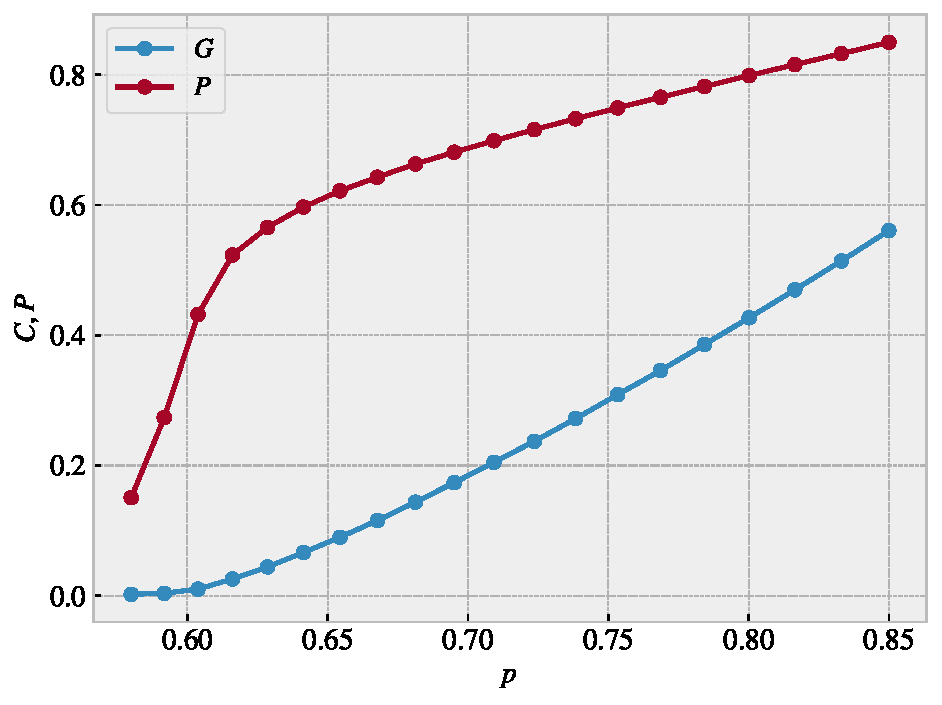
\includegraphics[width=\linewidth]{figures/GP(p).pdf}
  \caption{Conductance G(p,L) and density of spannig cluster $P(p,L)$ for $L = 400$ and 20 logaritmic distributed points for $p \in [0.58, 0.85]$. We used anaverage value over 100 MC cycles for each value of $p$.}
  \label{fig:GP(p)}
\end{figure}

\section{Scaling arguments for conductance and conductivity}
For an infinite system ($L\to\infty$) we cannot define a cunductance $G$ but must describe the system by its conductivity. In the special case of two dimensions the conductance and condutivity is the same:
\begin{align*}
  g = L^{2-2}G = G
\end{align*}
For an infinte system we have no spanning cluster for $p < p_c$, and thus no $g = 0$. When p is close to 1, the density of the spanning cluster will be proportional to to $p$. Can be showed with taylor expansion??:
\begin{align*}
  P(p) &= (p-p_c)^{\beta} \\
  T(P(p), a = 1) &= (1-P_c)^{\beta} + \beta(1-p_c)^{\beta-1}(p-1)
\end{align*}
Nonetheless we expect the conducance to be proportional to $p$ as well in this range. This could lead to the assumption that the density of the spanning cluster and the conductance of the sample is proportional to $p$ also when $p_c$ is close to $p_c$. However as we see on figure \ref{fig:GP(p)} this is clearly not the case when $p$ approach $p_c$.\par
The explanation for this lies in the fact that it is only th backbone that contributes to the conductance and not the dangling ends. We have found that the mass-scaling exponent of the backbone $D_B$, is smaller than the mass-scaling exponent for the spanning cluster $D$. This is the reason for the difference in the behaviour between $P(p)$ and $G(p)$ for $p$ close to $p_c$\par
We use the same scaling techniques, used to find the behaviour of $P(p,L)$, to develop a theory for the conductance $G(p,L)$. Instead of describing the cunductance as a function of $p$ we can use the correlation length (typical size?) $\xi$ such that
\begin{align*}
  G(p,L) = G(\xi,L)
\end{align*}
Second we realize that we want to describe the system for $p > p_c$. We will adress two limits: When $\xi \ll L$ and $\xi \gg L$ at $p_c$.

\subsection{Scaling for $\xi \ll L$ }
For $\xi \ll L$, we know that over length scales larger than $\xi$, the system is effectively homegenoues. We can see this by subdividing the system into cells of size $\xi$, giving us a total of $(L/\xi)^d$ cells. For a homogeneous system of $l^d$ boxes with size $l$, we know that the conductance $G$ of the whole system is $G = l^{d-2}G_l$, where $G_l$ is the conductance of a single box. We apply the same principle to this system and get:
\begin{align*}
  G(\xi,L) = \left(\frac{L}{\xi}\right)^{d-2}G(\xi, \xi)
\end{align*}
where we have written $G(\xi, \xi) =  G(\xi, L=\xi)$ for the conductivity within the box, which is the conductance of a system where the correlation length is $\xi$ and $L = \xi$. From \ref{eq:G_electric} we get the conductivity
\begin{align}
  g(\xi, L) = L^{-(d-2)} G(\xi,L) = \frac{G(\xi, \xi)}{\xi^{d-2}}
  \label{eq:g(xi,L)}
\end{align}
We then have to consider what is $G(\xi, \xi)$? We know that a system with correlation length equal to the system size is indistinguishable from a system at $p = p_c$ and $G(\xi, \xi)$ must therefore be the cunductance of the spanning cluster at $p=p_c$ in a system of size $L = \xi$. Let us therefore find the conductance of a finite system of size $L$ at the percolation threshold.
\subsection{Conductance of the spanning cluster}
We now adress the conducance $G(\infty, L)$ of the spanning cluster at $p=p_c$. The spanning cluster consist of the backbone and the dangling ends, but only the backbone will contribute to the conductivity. The backbone can be described by the blob model: The backbone consists of blobs of bonds in parallel, and links of singly connected bonds beetween them. \par
Our work flow is:
\begin{enumerate}
  \item Start form a scaling ansatz of the conductance
  \item derive the consequences
  \item compare with data and check for consistency
\end{enumerate}
This will validate (to be precisxe: at least not invalidate) the hypothesis/ansatz. Our scaling ansatz is that the conductance of the system of size $L$ at $p_c$ can be described by the scaling exponent $\zetaR$:
\begin{align}
  G(\infty, L) \propto L^{-\zetaR}
  \label{eq:zeta_ansatz}
\end{align}
We know try to investegate the bounds of the scaling ansatz.

\subsubsection{Lower bound of ansatz}
We know that the spanning cluster consists of blobs in series with single connected bonds. Thus the resistance $R = 1/G$ of the spannig cluster is given as:
\begin{align*}
  1/G = R = R_{SC} + R_{blob}
\end{align*}
where $R_{SC}$ is the resistance of the single connected bonds and $R_{blob}$ the resistance of the blobs. This implies that $R > R_{SC}$. Since the single connected bonds consist of sinlge sites connected in series we have
\begin{align*}
  R_{SC} = R_{SB}\cdot M_{SC}
\end{align*}
where $R_{SB}$ is the resistance of a single bond and $M_{SC}$ is the number of single connected bonds. This gives
\begin{align*}
  R > R_{RC} = R_{SC}M_{SC} \\
  R > M_{SC}
\end{align*}
where we used that the conductivity of an open bond is defined to be 1. such that $R_{SB} = 1/G_{SB} = 1$. We know that $M_{SC} \propto L^{D_{SC}}$, and from the ansatz \ref{eq:zeta_ansatz} we have $R \propto L^{\zetaR}$ which give:
\begin{align*}
  L^{\zetaR} &\ge L^{D_{SC}}  \\
   \zetaR &\ge D_{SC}
\end{align*}
We have know found a lower bound for $\zetaR$

\subsubsection{Upper bound of ansatz}
We find the upper bound by examinating the minimal path. The resistance of the spannign cluster will be smaller or equal to the resistance of the minimal path. This is beacause the spanning cluster will have som regions with blobs where the bonds are in parallel. Adding parallel bonds will always lower the resistance (see proof in appendix). Since the minimal path is a seris of resistances in series, the total resistance of the minimal path is the mass $M_{min}$ of the minimal path multiplied with by the resistance of a single bond. We get
\begin{align*}
  L^{\zetaR} \propto R &\le M_{min} \propto L^{D_{min}} \\
  \zetaR &\le D_{min}
\end{align*}
This is the upper limit.


\subsubsection{Combinning bounds}
We have then demonstated/proved the scaling relation
\begin{align*}
  D_{SC} \le \zetaR \le D_{min}
\end{align*}
Since the scaling of $R$ is bounded by two power-laws it can be shown mathematically that $R$ must also be a power-law, where the exponents are within the the given bounds. For high dimensionality the probaility of loops will be low and hence blobs will be unlikely. In this case we get
\begin{align*}
  D_{SC} = \zetaR = D_{min} = D_{max}
\end{align*}

\subsubsection{Conductivity ofr $p > p_c$}
We now established that
\begin{align*}
  G(\infty, L) \propto L^{-\zetaR}, \qquad when L \le \xi
\end{align*}
We use this to find an expression for $G(\xi, \xi)$, which is the conductance of the spanning cluster at $p = p_c$ in a system of size $L=\xi$. Therefore we have
\begin{align*}
  G(\xi, \xi) \propto \xi^{-\zetaR}
\end{align*}
We insert this into \ref{eq:g(xi,L)} and get
\begin{align*}
  g = \frac{G(\xi, \xi)}{\xi^{d-2}} &\propto \xi^{-(d-2+\zetaR)} \\
  &\propto (p-p_c)^{\nu(d-2+\zetaR)} \\
  &= (p-p_c)^{\mu}
\end{align*}
where we used $\xi \propto |p-p_c|^{-\nu}$ and introduced
\begin{align*}
  \mu = \nu(d-2+\zetaR)
\end{align*}
We notice that for two-dimensional perculation, any value of $\zetaR > 1/\nu$ will lwad to $\mu > 1$, which we observed in figure \ref{fig:GP(p)}. The exponent $\mu$ is bigger than 1, which is significally bigger than $\beta$ ($= 5/36$ for 2D), that describes the mass of the spannig cluster.

\section{Finding mu}

\begin{figure}[H]
  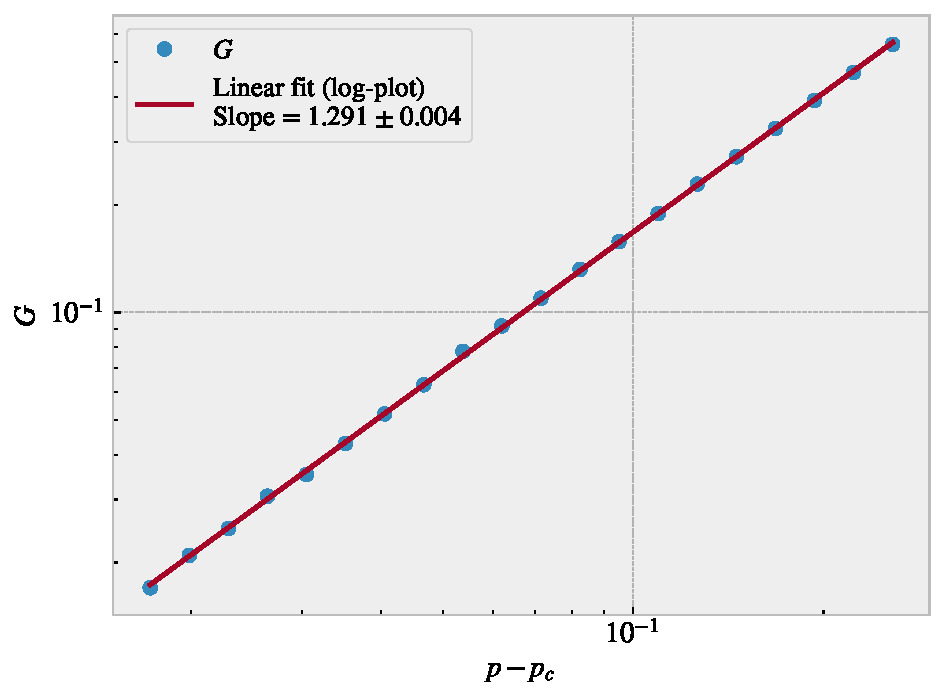
\includegraphics[width=\linewidth]{figures/mu.pdf}
  \caption{$G$ as a function of $p-p_c$ on a logaritmic plot. By finding the slope we estimate $\mu$}
  \label{fig:mu}
\end{figure}
From this we find
\begin{align*}
  \mu = 1.291 \pm 0.004
\end{align*}




The given estimate for $\mu$ according to \cite{textbook} is $\mu = 1.30$ giving a relative error of
\begin{align*}
  \eta_\mu= \left|\frac{1.30 - 1.291}{1.30}\right| = 0.007
\end{align*}


\clearpage


\section{Generelt bevis for at parallelforbunde bonds gir mindre mostand en minimum path.}
Vi antar at vi har en blob som forbinner to single connected blobs med $N$ forkjellige parallelforbunde veier med antall sites $M_1, M_2, \hdots, M_N$. Vi antar at konduktansen for hver av disse er $G_s=1$ og da har vi at motstanden i hvert site er $R_s = 1/G_s = 1$. Den totale motstand i bloben er git som
\begin{align*}
  \frac{1}{R} = \frac{1}{R_1} + \frac{1}{R_2} + \hdots + \frac{1}{R_N}
\end{align*}
Motstanden i hver forbinnelse er gitt som
\begin{align*}
 R_i = M_iR_s = M_i
\end{align*}
og vi får derved
\begin{align*}
 \frac{1}{R} = \frac{1}{M_1} + \frac{1}{M_2} + \hdots + \frac{1}{M_N}
\end{align*}
Vi definerer $M_min$ som den vei med korteste lengde $M_i$. Da har vi ulikhetet:
\begin{align*}
   \frac{1}{R} = \frac{1}{M_1} + \frac{1}{M_2} + \hdots + \frac{1}{M_N} \le \frac{N}{M_{min}} = \frac{N}{R_{min}}
\end{align*}
Dette gir den nedre grense
\begin{align*}
 R \ge \frac{1}{N} R_{min}
\end{align*}
Vi finner den øvre grense ved å se på hva som skjer dersom alle veiene untatt den minimale path blir veldig store:
\begin{align*}
 \lim_{M_{i\ne min}\to \infty} \frac{1}{R} = \frac{1}{\frac{1}{M_{min}} + (N-1)\frac{1}{0}} = M_{min} = R_{min}
\end{align*}
Da har vi vist følgende grenser:
\begin{align*}
 \frac{1}{N} R_{min} \le R \le R_{min}
\end{align*}

% \section{Notes}
% Vi har
% \begin{align*}
%   \text{serie:} \quad &R = R_1 + R_2 \\
%   \text{parallel:} \quad &\frac{1}{R} = \frac{1}{R_1} + \frac{1}{R_2}
% \end{align*}
% Antar at spanning cluster deler seg i to veie med en gang slik at
% \begin{align*}
%   R_{SP} = R_{\parallel} = \frac{1}{\frac{1}{R_1} + \frac{1}{R_2}}
% \end{align*}
% der $R_p$ har motstanden over de parallelforbunde veie med motstand $R_1$ og $R_2$ \par
% Den minimale path er en serieforbinnelse forbinnelse med $M_{min}$ sites slik at
% \begin{align*}
%   R_{min} = M_{min}R_{s}
% \end{align*}
% der $R_s$ er motstanden for hvert site gitt som $R_s = 1/G_s = 1$, der vi har brukt $G_s =1$. Vi finner for $R_p$:
% \begin{align*}
%   R_{\parallel} &= \frac{1}{\frac{1}{R_1} + \frac{1}{R_2}} \\
%   &= \frac{1}{\frac{1}{M_1R_s} + \frac{1}{M_2R_s}} \\
%   &= \frac{1}{\frac{1}{M_1} + \frac{1}{M_2}}
% \end{align*}
% Vi vet at $M_1, M_2 \ge M_{min}$ slik at:
% \begin{align*}
%     \frac{1}{M_1} + \frac{1}{M_2} \le \frac{1}{M_{min}} + \frac{1}{M_{min}}
% \end{align*}
% da får vi
% \begin{align*}
%   R_p = R_{tot} = \frac{1}{\frac{1}{M_1} + \frac{1}{M_2}} &\ge \frac{1}{\frac{1}{M_{min}} + \frac{1}{M_{min}}} \\
%   &= \frac{M_{min}}{2} = \frac{1}{2}R_{min}
% \end{align*}
% Hvis $M_2 \to \infty$ har vi:
% \begin{align*}
%   \lim_{M_2 \to \infty} R_{tot} = \frac{1}{\frac{1}{M_1} + 0} = M_1 = R_1
% \end{align*}
% Altså må vi ha
% \begin{align*}
%   \frac{1}{2} R_{min} \le R_{tot} \le R_{min}
% \end{align*}
%



% \section{Notes II}
% Fortsetter fra tidligere eksempel og spenningsforskjell over spanning cluster $V = 1$. I serie har vi:
% \begin{align*}
%   V = RI = I(R_1 + R_2 + \hdots)
% \end{align*}
% I parallel har vi
% \begin{align*}
% I &= I_1 + I_2 + \hdots \\
% &= \frac{V}{R_1} + \frac{V}{R_2} + \hdots \\
% &= V(\frac{1}{R_1} + \frac{1}{R_2} + \hdots)
% \end{align*}
% Vi sier at vi har to veie med modstand 1 og 2, der 1 tilsvarer minimale path. Da har vi samlet strøm:
% \begin{align*}
%   I_1 &= I_{min} = \frac{V}{R_1} = \frac{V}{M_1} \\
%   I_2 &= \frac{V}{M_2} = \frac{V}{M_2}
% \end{align*}
% Vi vet at $M_2 \ge M_1 = M_{min}$
% \begin{align*}
%   R_{tot} = \frac{V}{I} &= \frac{V}{I_1 + I_2} \\
%   &=  \frac{V}{\frac{V}{M_1} + \frac{V}{M_2}} \\
%   &= \frac{1}{\frac{1}{M_1} + \frac{1}{M_2}} \ge \frac{1}{\frac{1}{M_1} + \frac{1}{M_1}} \\
%   &= \frac{1}{2}M_1 = \frac{1}{2}R_1
% \end{align*}
% Hvis $M_2 \to \infty$ har vi
% \begin{align*}
%   \lim_{M_2 \to \infty} R_{tot} = \frac{1}{\frac{1}{M_1} + 0} = M_1 = R_1
% \end{align*}

\clearpage
\begin{thebibliography}{9}
  \bibitem{textbook} A.M. Sørensen, 2020, Percolation theory using Python, 20/04/2020, Department of Physics, University of Oslo. Availiable from: \url{https://www.uio.no/studier/emner/matnat/fys/FYS4460/v21/notes/book.pdf}
\end{thebibliography}

\end{document}
